\documentclass[11pt,a4paper]{report}
\usepackage{graphicx}
\graphicspath{{./images/}}
\usepackage[utf8]{inputenc}
\usepackage{amsmath}
%\usepackage{tabto}
\usepackage{amsfonts}
\usepackage{amssymb}
\usepackage{amsthm}
\usepackage{xcolor}
\usepackage{tabularx}
\usepackage{booktabs}
\usepackage[margin=1in]{geometry}

\usepackage[colorlinks=true,          % link colors, set to 'false' for print version
            linkcolor=blue,
            citecolor=red,
            urlcolor=blue]{hyperref}
            

%\setlength{\topmargin}{30mm}
%\addtolength{\topmargin}{-1in}
%\addtolength{\topmargin}{-\headsep}
%\addtolength{\topmargin}{-\headheight}
%\addtolength{\topmargin}{-\topskip}

%\setlength{\textheight}{270mm}
%\addtolength{\textheight}{\topskip}
%\addtolength{\textheight}{-\footskip}
%\addtolength{\textheight}{-30pt}

%\setlength{\oddsidemargin}{-1in}
%\addtolength{\oddsidemargin}{20mm}
%\setlength{\evensidemargin}{\oddsidemargin}

%\setlength{\textwidth}{170mm}

\newtheorem{defn}{Definition}[section]
 \newtheorem{thm}{Theorem}[section]
 \newtheorem{Lemma}{Lemma}[section]
 \newtheorem{Claim}{Claim}[section]
 \newtheorem{Prop}{Proposition}[section]
  \theoremstyle{definition}\newtheorem{Ex}{Example}[section]
 \newtheorem{Cor}{Corollary}[section]
 \newtheorem{claim}{Claim}[section]
 \newtheorem{conj}{Conjecture}  

\usepackage {amsfonts,amssymb}
%\usepackage{mathbbol}
\usepackage{latexsym}
\usepackage{mathrsfs}
\input xy
\xyoption{all}

\newcommand {\op}{\mathcal{O}\mathfrak{p}}
\newcommand {\Def}{\textrm{Def}}
\newcommand {\MC} {\textrm{MC}}
\newcommand {\Art}{\textrm{Art}_\CC}
\newcommand {\Kur}{\textrm{Kur}}
\newcommand {\LG} {^LG}
\newcommand{\fart}{\textrm{FArt}_\CC}
\newcommand{\fun}{\textrm{Fun}}
\newcommand{\sets}{\textrm{Sets}}
\newcommand{\tops}{\textrm{Top}}

\newcommand {\BB}{\mathbb{B}}
\newcommand {\CC}{\mathbb{C}}
\newcommand {\FF}{\mathbb{F}}
\newcommand {\KK}{\mathbb{K}}
\newcommand {\MM}{\mathbb{M}}
\newcommand{\NN}{\mathbb{N}}
\newcommand {\PP}{\mathbb{P}}
\newcommand{\QQ}{\mathbb{Q}}
\newcommand {\RR}{\mathbb{R}}
\newcommand {\SSS}{\mathbb{S}}
\newcommand {\VV}{\mathbb{V}}
\newcommand {\HH}{\mathbb{H}}
\newcommand {\WW}{\mathbb{W}}
\newcommand{\YY}{\mathbb{Y}}
\newcommand{\ZZ}{\mathbb{Z}}


\newcommand {\bal}{\boldsymbol{\alpha}}
\newcommand {\bbe}{\boldsymbol{\beta}}
\newcommand {\bga}{\boldsymbol{\gamma}}
\newcommand {\bmu}{\boldsymbol{\mu}}
\newcommand {\bom}{\boldsymbol{\omega}}
\newcommand {\bth}{\boldsymbol{\theta}}
\newcommand {\bph}{\boldsymbol{\phi}}
\newcommand {\bdh}{\boldsymbol{h}}
\newcommand {\bdk}{\boldsymbol{k}}
\newcommand {\bdE}{\boldsymbol{E}}
\newcommand {\bdU}{\boldsymbol{U}}
\newcommand {\bdP}{\boldsymbol{P}}
\newcommand {\ba}{{\bf a}}
\newcommand {\bb}{{\bf b}}
\newcommand {\bc}{{\bf c}}
\newcommand {\bd}{{\bf d}}
\newcommand {\bg}{{\bf g}}
\newcommand {\be}{{\bf e}}
\newcommand {\bdf}{{\bf f}}
\newcommand {\bp}{{\bf p}}
\newcommand {\bq}{{\bf q}}
\newcommand {\bv}{{\bf v}}
\newcommand {\bh}{{\bf h}}
\newcommand {\bk}{{\bf k}}
\newcommand {\br}{{\bf r}}
\newcommand {\bdu}{{\bf u}}
\newcommand {\bdv}{{\bf v}}
\newcommand {\bi}{{\bf i}}
\newcommand {\bj}{{\bf j}}
\newcommand {\bn}{{\bf n}}
\newcommand {\bs}{{\bf s}}
\newcommand {\bt}{{\bf t}}
\newcommand {\bu}{{\bf u}}
\newcommand {\bw}{{\bf w}}
\newcommand {\bx}{{\bf x}}
\newcommand{\by}{{\bf y}}
\newcommand {\bz}{{\bf z}}
\newcommand {\bB}{{\bf B}}
\newcommand{\bD}{{\bf D}}
\newcommand {\bE}{{\bf E}}
\newcommand {\bF}{{\bf F}}
\newcommand {\bG}{{\bf G}}
\newcommand {\bH}{{\bf H}}
\newcommand {\bK}{{\bf K}}
\newcommand {\bL}{{\bf L}}
\newcommand {\bM}{{\bf M}}
\newcommand {\bN}{{\bf N}}
\newcommand {\bO}{{\bf O}}
\newcommand {\bP}{{\bf P}}
\newcommand {\bQ}{{\bf Q}}
\newcommand {\bR}{{\bf R}}
\newcommand {\bT}{{\bf T}}
\newcommand {\bS}{{\bf S}}
\newcommand {\bU}{{\bf U}}
\newcommand {\bV}{{\bf V}}
\newcommand {\bW}{{\bf W}}
\newcommand {\bgamma}{\boldsymbol\gamma}
\newcommand {\bdelta}{\boldsymbol\delta}
\newcommand {\bDelta}{\boldsymbol\Delta}
%\newcommand{\qed}{{\ \bf qed}}

\newcommand {\rroot}{\mathbf{root}}
\newcommand {\coroot}{\mathbf{coroot}}
\newcommand {\weight}{\mathbf{weight}}
\newcommand {\coweight}{\mathbf{coweight}}
 \newcommand{\higgs}{\textrm{Higgs}}
\newcommand{\bun}{\textrm{Bun}}
\newcommand{\rk}{\textrm{rk}}
\newcommand{\ext}{\textrm{Ext}}
% \newcommand {\id}{\mathbb{1}}
% Use \id if using mathbbol instead of amssymb
\newcommand{\range}{\textrm{Range}}
\newcommand{\arccot}{\textrm{arccot}}

\newcommand{\thickslash}{\mathbin{\!\!\pmb{\fatslash}}}


\newcommand{\cA}{\mathcal{A}}
\newcommand{\cB}{\mathcal{B}}
\newcommand{\cC}{\mathcal{C}}
\newcommand{\cD}{\mathcal{D}}
\newcommand{\cE}{\mathcal{E}}
\newcommand{\cF}{\mathcal{F}}
\newcommand{\cG}{\mathcal{G}}
\newcommand{\cH}{\mathcal{H}}
\newcommand{\cI}{\mathcal{I}}
\newcommand{\cJ}{\mathcal{J}}
\newcommand{\cK}{\mathcal{K}}
\newcommand{\cL}{\mathcal{L}}
\newcommand {\cM}{\mathcal{M}}
\newcommand {\cN}{\mathcal{N}}
\newcommand {\cO}{\mathcal{O}}
\newcommand{\cP}{\mathcal{P}}
\newcommand{\cQ}{\mathcal{Q}}
\newcommand{\cR}{\mathcal{R}}
\newcommand{\cS}{\mathcal{S}}
\newcommand{\cT}{\mathcal{T}}
\newcommand{\cU}{\mathcal{U}}
\newcommand{\cV}{\mathcal{V}}
\newcommand{\cW}{\mathcal{W}}
\newcommand{\cX}{\mathcal{X}}
\newcommand{\cY}{\mathcal{Y}}
\newcommand{\cZ}{\mathcal{Z}}

\newcommand{\loc}{\mathcal{L}oc}
\newcommand{\Loc}{\textrm{Loc}}
\newcommand{\cih}{\mathpzc{h}}
\newcommand{\cx}{\mathpzc{x}}
\newcommand{\cy}{\mathpzc{y}}
\newcommand{\ce}{\mathpzc{e}}
\newcommand{\cf}{\mathpzc{f}}
\newcommand{\cl}{\mathpzc{l}}




 




\newcommand{\scA}{\mathscr{A}}
\newcommand{\scB}{\mathscr{B}}
\newcommand{\scC}{\mathscr{C}}
\newcommand{\scD}{\mathscr{D}}
\newcommand{\scE}{\mathscr{E}}
\newcommand{\scF}{\mathscr{F}}
\newcommand{\scG}{\mathscr{G}}
\newcommand{\scH}{\mathscr{H}}
\newcommand{\scI}{\mathscr{I}}
\newcommand{\scJ}{\mathscr{J}}
\newcommand{\scK}{\mathscr{K}}
\newcommand{\scL}{\mathscr{L}}
\newcommand{\scM}{\mathscr{M}}
\newcommand{\scP}{\mathscr{P}}
\newcommand{\scR}{\mathscr{R}}
\newcommand{\scO}{\mathscr{O}}
\newcommand{\scS}{\mathscr{S}}
\newcommand{\scT}{\mathscr{T}}
\newcommand{\scU}{\mathscr{U}}
\newcommand{\scV}{\mathscr{V}}
\newcommand{\scW}{\mathscr{W}}
\newcommand{\scX}{\mathscr{X}}
\newcommand{\scY}{\mathscr{Y}}
\newcommand{\scZ}{\scZ}

\newcommand{\uR}{\underline{\mathbb{R}}}
\newcommand {\uC}{\underline{\mathbb{C}}}


\newcommand{\fh}{\mathfrak{h}}
\newcommand{\fa}{\mathfrak{a}}
\newcommand{\fb}{\mathfrak{b}}
\newcommand{\fc}{\mathfrak{c}}
\newcommand{\fg}{\mathfrak{g}}
\newcommand{\fk}{\mathfrak{k}}
\newcommand{\fl}{\mathfrak{l}}
\newcommand{\fm}{\mathfrak{m}}
\newcommand{\fn}{\mathfrak{n}}
\newcommand{\fo}{\mathfrak{o}}
\newcommand{\fp}{\mathfrak{p}}
\newcommand{\fr}{\mathfrak{r}}
\newcommand{\fs}{\mathfrak{s}}
\newcommand{\fsu}{\mathfrak{su}}
\newcommand{\ft}{\mathfrak{t}}
\newcommand{\slt}{\mathfrak{sl}_2(\CC)}
\newcommand{\sln}{\mathfrak{sl}(n)}
\newcommand{\fsl}{\mathfrak{sl}}
\newcommand{\fu}{\mathfrak{u}}
\newcommand{\fv}{\mathfrak{v}}
\newcommand{\fx}{\mathfrak{x}}
\newcommand{\fy}{\mathfrak{y}}
\newcommand{\fz}{\mathfrak{z}}
\newcommand{\fA}{\mathfrak{A}}
\newcommand{\fB}{\mathfrak{B}}
\newcommand{\fD}{\mathfrak{D}}
\newcommand{\fM}{\mathfrak{M}}
\newcommand{\fR}{\mathfrak{R}}
\newcommand {\fU}{\mathfrak{U}}
\newcommand {\fV}{\mathfrak{V}}
\newcommand {\fW}{\mathfrak{W}}
\newcommand{\fX}{\mathfrak{X}}
\newcommand{\faff}{\mathfrak{aff}}

\newcommand{\Aff}{\textrm{Aff}}

\newcommand{\sym}{\textrm{Sym}}

\newcommand {\dbar}{\overline{\partial}}
\newcommand {\zbar}{\overline{z}}
\newcommand {\zvec}{\underline{z}}
\newcommand {\dzbar}{d\overline{z}}
\newcommand {\Nbar}{\overline{N}}
\newcommand {\Kbar}{\overline{K}}
\newcommand{\diff}{\textrm{Diff}}

%\newcommand {\hom}{\textrm{Hom}}

\newcommand{\mhom}{\textrm{Hom}}
\newcommand {\mend}{\textrm{End}}
\newcommand {\misom}{\textrm{Isom}}
\newcommand {\maut}{\textrm{Aut}}
\newcommand{\pr}{\textrm{pr}}

\newcommand {\sisom}{\underline{Isom}}
\newcommand {\saut}{\underline{Aut}}
\newcommand {\shom}{\textrm{\underline{Hom}}}
\newcommand {\send}{\underline{End} }

\newcommand{\dra}{M^{an}_{DR}(X,G)}
\newcommand{\dr}{M_{DR}(X,G)}

\newcommand {\ad}{\textrm{ad} }
\newcommand{\Ad}{\textrm{Ad}}

\newcommand{\lspan}{\textrm{span}}
\newcommand{\img}{\textrm{Im }}
\newcommand{\spec}{\textrm{Spec }}
\newcommand{\specan}{\textrm{Spec}^{an}}
\newcommand{\gspec}{\underline{\textrm{Spec }}}
\newcommand {\cok}{\textrm{coker}}
\newcommand{\tot}{\textrm{tot }}
\newcommand{\tildel}{\widetilde{\delta}}
\newcommand{\ctimes}{\otimes_\CC}
\newcommand{\sotimes}{\otimes_{\cO_X}}
\newcommand{\pic}{\textrm{Pic}}
\newcommand{\tr}{\textrm{tr }}

\newcommand  {\eps}{\varepsilon}
\newcommand {\kap}{\varkappa}
\newcommand {\io}{\iota}
\newcommand {\fii}{\varphi}

\newcommand{\Higgs}{{\bf Higgs}}
\newcommand{\Bun}{{\bf Bun}}
\newcommand{\gHiggs}{\op{\boldsymbol{\mathcal{H}iggs}}}
\newcommand{\Prym}{{\bf Prym}}
\newcommand{\Jac}{{\bf Jac}}
%\newcommand{\bh}{\boldsymbol{h}}
%\newcommand{\bH}{\boldsymbol{\mathcal{H}}}
\newcommand{\rts}{{\sf root}}
\newcommand{\wts}{{\sf weight}}
\newcommand{\crts}{{\sf coroot}}
\newcommand{\cwts}{{\sf coweight}}
\newcommand{\chr}{{\sf char}}
\newcommand{\cchr}{{\sf cochar}}

\newcommand{\Aut}{\textrm{Aut}}
\newcommand{\Der}{\textrm{Der}}
\newcommand{\spin}{\textrm{Spin}}
\newcommand{\spinc}{\textrm{Spin}^c}
%\newcommand{\U}{\boldsymbol{U(1)}}

\newcommand{\Mat}{\textrm{Mat}}

\newcommand{\hookr}{\hookrightarrow}

%%%%%%%%%%%%%%%%%%%%%%%%%%%%%%%%%%%%%%%%%%%%%%%%%%%%%%%%%%%%%%%%%%%%%%%%%
% Long exact sequence macro
%%%%%%%%%%%%%%%%%%%%%%%%%%%%%%%%%%%%%%%%%%%%%%%%%%%%%%%%%%%%%%%%%%%%%%%%%

\newcommand{\les}[9]{
\xymatrix{
 0 \ar[r] & {#1} \ar[r]  &  {#2} \ar[r]  &  {#3}
\ar@{->}`r/10pt[d] `[l] `^dl[dlll]  `^dr/10pt[dll]    [dll] \\
 &  {#4} \ar[r] & {#5} \ar[r] & {#6}
\ar@{->}`r/10pt[d] `[l] `^dl[dlll]  `^dr/10pt[dll]    [dll] \\
 & {#7} \ar[r]  & {#8} \ar[r] & {#9}
\ar@{->}`r/10pt[d] `[l] `^dl[dlll]  `^dr/10pt[dll]    [dll] \\
 & 0 \ar[r] & \cdots & }
}


%%%%%%%%%%%%%%%%%%%%%%%%%%%%%%%%%%%%%%%%%%%%%%%%%%%%%%%%%%%%%%%%%%%%%%%%%

\newcommand{\lestwo}[9]{
\xymatrix{     
 0 \ar[r] & {#1} \ar[r]  &  {#2} \ar[r]  &  {#3} 
\ar@{->}`r/10pt[d] `[l] `^dl[dlll]  `^dr/10pt[dll]    [dll] \\
 &  {#4} \ar[r] & {#5} \ar[r] & {#6} 
\ar@{->}`r/10pt[d] `[l] `^dl[dlll]  `^dr/10pt[dll]    [dll] \\
 & {#7} \ar[r]  & {#8} \ar[r] & {#9} }
}

%%%%%%%%%%%%%%%%%%%%%%%%%%%%%%%%%%%%%%%%%%%%%%%%%%%%%%%%%%%%%%%%%%%%%%%%%
% Long exact sequence macro
%%%%%%%%%%%%%%%%%%%%%%%%%%%%%%%%%%%%%%%%%%%%%%%%%%%%%%%%%%%%%%%%%%%%%%%%%

\newcommand{\lesthree}[5]{
\xymatrix{     
 0 \ar[r] & {#1} \ar[r]  &  {#2} \ar[r]  &  {#3} 
\ar@{->}`r/10pt[d] `[l] `^dl[dlll]  `^dr/10pt[dll]    [dll] \\
 &  {#4} \ar[r] & {#5} & }
}


%%%%%%%%%%%%%%%%%%%%%%%%%%%%%%%%%%%%%%%%%%%%%%%%%%%%%%%%%%%%%%%%%%%%%%%%%
% Long exact sequence macro
%%%%%%%%%%%%%%%%%%%%%%%%%%%%%%%%%%%%%%%%%%%%%%%%%%%%%%%%%%%%%%%%%%%%%%%%%

\newcommand{\lesfour}[8]{
\xymatrix{     
 0 \ar[r] & {#1} \ar[r]  &  {#2} \ar[r]  &  {#3} 
\ar@{->}`r/10pt[d] `[l] `^dl[dlll]  `^dr/10pt[dll]    [dll] \\
 &  {#4} \ar[r]^-{#8} & {#5} \ar[r] & {#6} 
\ar@{->}`r/10pt[d] `[l] `^dl[dlll]  `^dr/10pt[dll]    [dll] \\
 & {#7} \ar[r]  & \cdots  &  }
}

\newcommand{\equivclass}[1]{%
  #1/{\sim}%
}
\newcommand{\equivcls}[1]{%
  #1/\!{\sim}%
}

%


\include{biblio}

\title{Optimization over Grassmann Manifolds}
\author{Author: Milos Vukadinovic}
\date{\parbox{\linewidth}{\centering%
  \endgraf\bigskip
  Advisor: Peter Dalakov \endgraf\medskip
  \bigskip
  Department\ of Mathematics,  \endgraf
  American University in Bulgaria \endgraf
  \bigskip
  \today}}
%\input{preamble}
\begin{document}
\maketitle

\begin{abstract}
We present optimization methods for functions whose domain lies on Grassmann Manifold.
Such functions are ubiquitous because data with subspace-structured features, orthogonality, or low-rank constraints can be naturally expressed using Grassmann manifold.
We consider two different representations of the Grassmann manifold: one as a quotient of Stiefel manifold and another as a set of projectors.
We develop Grassmannian gradient descent and Grassmannian Newton method on these representations.
We demonstrate the efficiency of Grassmannian algorithms by optimizing Rayleigh quotient and conclude that our algorithms converge faster, generalize better and perform as well as the best-known problem-specific algorithms. 
\end{abstract}

\setcounter{tocdepth}{1}
\tableofcontents
\chapter{Introduction}
\textit{An overview of the topic} \newline

Constrained optimization is the process of optimizing an objective function with respect to some variables with the presence of constraints on those variables.
In our paper, we consider geometric constraints, which express that the solution of the optimization problem lies on a manifold.
Specifically, we consider problems where the solution lies on a Grassmann manifold.
Grassmann manifold $G(p,n)$ is a set of $p$ dimensional subspaces in a higher $n$ dimensional space.
Such problems are ubiquitous, because data with subspace-structured features, ortogonality constraints or low-rank constrains can be naturally expressed using Grassmann manifold.
For example symmetric eigenvalue problems, nonlineareigenvalue problems, electronic structures computations, and signal processing can all be optimized over $G(p,n)$.
In our paper, we first show how Grassmann manifold can be considered as a quotient manifold and as a set of projectors. Then, we develop Gradient Descent and Newton's algorithm on Grassmann manifold, and study its applications to eigenvalue and eigenvector computations.

\textit{Prior Research} \newline
A framework for algorithms involving these constraints was first introduced by Edelman et al \cite{edelman_geometry_1998} .
They used a quotient manifold representation to develop Newton algorithm, which inspired a line of works that improve the algorithm or find a different application \cite{hamm_grassmann_nodate} \cite{ma_flag_2020} \cite{johnsson_optimization_nodate} \cite{tripuraneni_averaging_2018}.
Set of projectors approach was introduced by Helmke et al \cite{helmke_newtons_2007}, and used to develop Newton algorithms on Grassman and Lagrange-Grassman manifolds.
While the mentioned representations (set of projectors and quotient manifold) are employed in our paper, they are certainly not exhaustive.
For example, Lai et al \cite{lai_simpler_2020} represent Grassmann manifold as symmetric ortogonal matrices of trace $2k -n$.
Extensive resources for learning about Riemmannian optimization are books by Absil \cite{AbsMahSep2008} and Boumal \cite{boumal2022intromanifolds}
Moreover, there are some programming frameworks for R, Python, Julia and Matlab that implemented grassmannian optimization such as GrassmannOptim \cite{adragni_grassmannoptim_2012}, and ManOpt \cite{JMLR:v17:16-177}.
The recent success of geometric deep learning \cite{DBLP:journals/corr/abs-2104-13478} \cite{masci_geodesic_2018}, 
shows the importance of exploiting the underlying geometric structure to improve learning.
Some attempts to construct a Grassmannian DNN have already been made \cite{zhang_grassmannian_2018} \cite{huang_building_2018}, but there are many challanges to overcome for them to appear in industry.
\textit{Rationale} \newline
There is a huge amount of digital data that we can use to extract valuable insights, and predictions.
Any time series data like stock price, electrocardiogram data or video data can be considered as points on Grassmann manifold.
Thus the development of grassmannian optimization algorithms will help us make new discoveries, reduce data size, and do it faster than classical optimization algorithms.
Moreover, by exploring the optimization algorithms on Grassmann manifold, we'll be taing a first step towards defining a Grassmannian deep neural network.
By embedding the geometry in neural network we will develop models with better accuracy and robustness. 
\newline
\textit{A thesis statement} \newline
Describe your contribution

\textit{Outline} \newline

\chapter{Sphere As Manifold}
\begin{defn}
     $(X,\mathcal{T})$ is a \textbf{locally Euclidean} topological space of dimension $n$  if $\forall \; p \in X \; \exists \; v \subseteq X$ which is homeomorphic to an open in $\RR^n$.
\end{defn}
\begin{defn}
      A \textbf{topological manifold} of dimension $n$ is a locally Euclidean space of $dim$ $n$ which is Hasudorff and has a countable base for its topology.
\end{defn}
\begin{defn}
      A \textbf{smooth atlas} is a collection of charts $\{ (v_{\alpha}, \varphi_{\alpha}) \}_{\alpha}$, $\bigcup_{\alpha} v_{\alpha} = X$, s.t. for any two charts $(v_{\alpha} , \varphi_{\alpha})$, and $(v_{\beta} , \varphi_{\beta})$
      the transition map $\varphi_{\alpha \beta} = \varphi_{\alpha} \circ \varphi_{\beta}^{-1} : \varphi_{\beta}(v_{\alpha} \cap v_{\beta}) \to \varphi_{\alpha}(v_{\alpha} \cap v_{\beta})$ is infinitely differentiable ($C^{\infty})$
\end{defn}
\begin{defn}
  A \textbf{smooth manifold} is a manifold together with a maximal atlas defined on it. We call the atlas maximal if is not contained in another atlas.
\end{defn}
\section{Sphere as a smooth manifold}
We will show that sphere $S^2$ is a smooth manifold. Let's denote a sphere as:
\begin{equation} \label{s2}
 M = S^2 = \{(x_1,x_2,x_3) \in \RR^3 \mid x_1^2 + x_2^2 + x_3^2 = 1 \} 
\end{equation}
Also, we define a disk with a center at $(x_0,y_0)$ and radius $\epsilon$ as:
$$ D_{\epsilon}(x_0,y_0) = \{(x,y) \in \RR^2 : (x-x_0)^2 + (y-y_0)^2 < \epsilon^2 \} $$

Thus we can cover the sphere with 6 charts and 6 functions, described as follows:
$$ u_i^{+} = S^2 \cap \{x_i > 0 \}, \quad u_i^{-} = S^2 \cap \{x_i < 0 \} $$
$$ \varphi_i^{+}: u_i^{+} \to D_{1}(0,0), \quad \varphi(x_1,x_2,x_3) = (\dots \hat{x_i} \dots)$$
$$ \varphi_i^{-}: u_i^{-} \to D_{1}(0,0), \quad \varphi(x_1,x_2,x_3) = (\dots \hat{x_i} \dots)$$
Then the atlas covering the sphere is:
$$ A_1 = \{(u_i^{\pm},\varphi_i^{\pm}) : i \in I \}, \quad I = \{ 1,2,3 \} $$
For example $\varphi_3^{+}: u_3^{+} \to \RR^2, \quad \varphi_3^{+}(x_1,x_2,x_3) = (x_1,x_2,\hat{x_3}) =(x_1,x_2)$
\newline
\newline
We first show that a function $\varphi_3^{+}: u_3^{+} \to \RR$ is injective. Assume $\exists P_1$ and $P_2$ s.t. $P_1 = (p_1,p_2,p_3)$,
and $P_2 = (p_1\prime,p_2\prime,p_3\prime)$, $P_1 \neq P2$, and $f(P_1) = f(P_2) \iff  (p_1,p_2) = (p_1\prime, p_2\prime)$
\newline
Because $P_1$ and $P_2$ are the points on the sphere:
$p_3\prime = \pm \sqrt{1-p_1^2-p_2^2} \quad \pm p_3\prime = \pm \sqrt{1-p_1\prime^2-p_2\prime^2}$
Since $u_3^{+}$ has only positive numbers for a third coordinate $p_3 = p_3\prime \implies (p_1,p_2,p_3) = (p_1\prime,p_2\prime,p_3\prime) \implies P_1=P_2$, and we can conclude that $\varphi_3^{+}$ is injective.
\newline
\newline
To show that $\varphi_i^{\pm}$ is injective, we similarly assume that $ \exists P_1$ and $P_2$, $P_1 \neq P_2$ and 
$\varphi_i^{\pm}(P_1) = \varphi_i^{\pm}(P_2)$. Let $K= \{1,2,3\}/i$. Then $\forall k \in K, a_k= a_k\prime$ 
$\quad a_i = \pm \sqrt{1-\sum(a_k^2)} = a_i\prime$. Since $a_i$ and $a_i\prime$ are limited to only positive or only negative values  $P_1 = P_2$, and $\varphi_i^{\pm}$ is injective.
\newline
\newline
To prove surjectivity, consider $(\varphi_i^{\pm})^{-1}$ componentwise. It sends an arbitary point $(b_1,b_2) \in \RR^2$ to a point $(a_1,a_2,a_3) \in S^2$, or componentwise
\[
  a_j =
  \begin{cases}
                                   b_j & j<i \\
                                   \sqrt{1-b_1^2-b_2^2} & j=i \\
                                   b_{j-1} & j>i
  \end{cases}
\]
Since each component in both $S^2$ and the disk varies from $0$ to $1$, each point in the codomain is mapped to, and we have surjectivity for $\varphi_i^{\pm}$
\newline
\begin{Lemma}\label{contLemma}
  Let $f:U \subset \RR^n \to \RR^m $. Suppose the partial derivatives $\frac{\partial f_i}{\partial x_j}$ of $f$ all exist
  and are continuous in a neighbourhood of a point $x \in U$. Then $f$ is differentiable at $x$. 
\end{Lemma}
The function $\varphi_i$ is continous by \ref{contLemma} (polynomials are infinitely differentiable).
%We can easily check for continuity of $\varphi_i$ since for each open $ \beta_{\epsilon}(x_1,x_2) \in D_1 (0,0) \; \exists \; \beta_{\delta}(x_1,x_2,\sqrt{1-x_1^2-x_2^2}) \in S^2 $ 
%such that $\epsilon = (\epsilon_1,\epsilon_2) $ and $\delta = (\epsilon_1,\epsilon_2, \sqrt{1-\epsilon_1^2-\epsilon_2^2})$
%\newline
%Similarly $\varphi_i^{-1}$ is continuous because $\forall \beta_{\epsilon}(x,y,z) \in S^2 \; \exists \; \beta_{\delta}(x,y) \in D_1(0,0) $ where $\delta = (\epsilon_1, \epsilon_2)$ 
\newline
The space is Hausdorff since it is a subset of $\RR^3$, therefore $\varphi_{i}^{\pm}$ are homeomorphisms.
\newline
We now show that $A$ is a smooth atlas. First we consider the transition function $ \varphi_3 \; \circ \; \varphi_1^{-1}: u_1^{+} \to u_3^{+}$
$$(x,y) \to (\sqrt{x^2+y^2},x,y) \to (\sqrt{x^2+y^2},x)$$
But this is infinitely differentiable since it is a polynomial. Similarly, we can show that all transition functions are $C^{\infty}$.
This proves that the sphere is a smooth manifold, but there is also an alternative proof that uses fewer charts.
\section{Sphere as a smooth manifold using stereographic projection}
\textbf{Stereographic projection} is a map that will allow us to embed the sphere with smooth structure by using 2 charts.
\newline
\begin{figure}[h] \label{ster_proj}
    \centering
    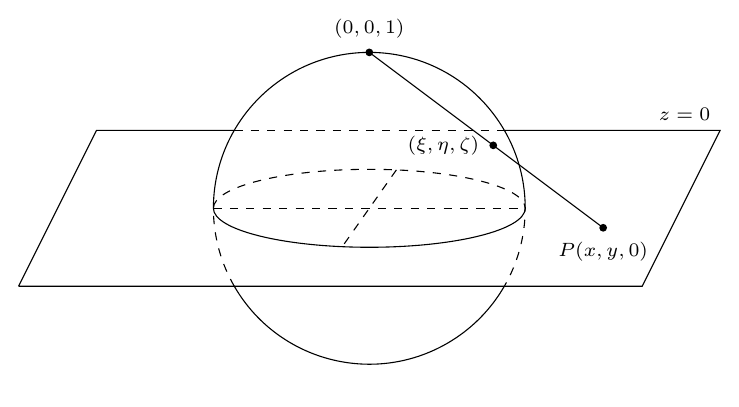
\includegraphics[width=0.90\textwidth]{stereographic_projection.png}
    \caption{Stereographic Projection Visualized}
\end{figure}
$$ v^{+} = S^2 \setminus \{(0,0,-1)\} \quad v^{-} = S^2 \setminus \{ (0,0,1) \} $$
We think of map $\phi^{-}$ as drawing a line through the point the north pole $(0,0,1)$ and $(x,y,z)$, then the output is the point where the line intersects z plane.
Similarly for $\phi^{+}$, we project from the south pole $(0,0,-1)$. We get the maps explicitly by parametrizing the line:
$$ l: (0,0,1) + t ((x_1,x_2,x_3) - (0,0,1)) =  (x_1 t,x_2 t, x_3 t-t+1) $$
$l$ intersects $x_3=0$ when $x_3t-t+1=$, thus $t = \frac{1}{(1-x_3)}$ It follows that the point of intersection is $(\frac{x_1}{1-x_3},\frac{x_2}{1-x_3},0)$
Similarly we can explicitly find $\phi^{+}$
$$ \phi_{+}: v^{+} \to \RR^2, \quad (x_1,x_2,x_3) \to (\frac{x_1}{1+x_3}, \frac{x_2}{1+x_3} )$$
$$ \phi_{-}: v^{-} \to \RR^2, \quad (x_1,x_2,x_3) \to (\frac{x_1}{1-x_3}, \frac{x_2}{1-x_3} )$$
We can find the inverses in the similar way.
Consinder points on the $z=0$ plane in $\RR^3$ $(\alpha, \beta, 0)$. We parametrize the line through this point and north pole:
$$ l: (0,0,1) + t((\alpha, \beta, 0 ) - (0,0,1)) = (\alpha t, \beta t, -t +1)$$
We need to see when are these points going to be on the sphere , i.e.
$$ (\alpha t)^2  + (\beta t)^2 + (-t +1)^2 = 1 $$
$$ \alpha^2 t^2 + \beta^2 t^2 + t^2 - 2t + 1 = 1 $$
$$ t^2 (\alpha^2 + \beta^2 +1 - \frac{2}{t} ) = 0 $$
$$ \therefore t = \frac{2}{\alpha^2 + \beta^2 +1 } $$
$$ \phi_{+}^{-1}:
\RR^2 \to v^{+} 
\quad (\alpha, \beta)  \to
( \frac{2 \alpha}{1+\alpha^2+\beta^2},
  \frac{2 \beta}{1+\alpha^2+\beta^2},
  - \frac{\alpha^2+\beta^2-1}{\alpha^2+\beta^2+1})
$$
$$ \phi_{-}^{-1}:
\RR^2 \to v^{-}
\quad (\alpha,\beta) \to
( \frac{2\alpha}{1+\alpha^2+\beta^2}, 
\frac{2\beta}{1+\alpha^2+\beta^2}, 
 \frac{\alpha^2 + \beta^2 -1}{\alpha^2+\beta^2+1} )
$$
Since we explicitly found an inverse, the function is bijection.
\newline
And it's easy to see that $\phi$ is continuous by lemma \ref{contLemma} (denom never zero)
Thus we equipped the sphere with the following atlas:
$$ A_2 = \{(v^{\pm},\phi_{\pm}) \} $$
We can check that the transition maps from $A_1$ to $A_2$ are smooth. \newline
First we check for $\varphi_3^{+} \circ \phi_{+}^{-1}$ where
$$ \varphi_3^{+}: S^2 \cap {x_3 > 0} = u_3^{+} \to D_1(0,0) \subset \RR^2 $$
$$ \phi_{+}^{-1}: \RR^2 \to v^{+} = S^2 \setminus \{ (0,0,-1) \} $$
Now, since we require that the domain of $\varphi_3^{+}$ is positive, the following is how our transition function will look like

$$\varphi_3^{+} \circ \phi_{+}^{-1}: D_1 (0,0) \to D_1(0,0), \quad \varphi_3^{+}( \phi_{+}^{-1}(x_1,x_2)) = (\frac{2x_1}{1+x_1^2+x_2^2}, \frac{2x_2}{1+x_1^2+x_2^2})$$

$$ \phi_{+}^{-1} \circ \varphi_3^{+}: D_1 (0,0) \to D_1(0,0), \quad  \phi_{+}(\varphi_3^{+}((x_1,x_2) )^{-1}) = (\frac{x_1}{1+\sqrt{1-x_1^2-x_2^2}}, \frac{x_1}{1+\sqrt{1-x_1^2-x_2^2}})$$
It is continuous componentwise and thus smooth.
Next, we list the domain and the image of the rest of transition maps.
$$\varphi_3^{-} \circ \phi_{+}^{-1}: \RR^2 \setminus \bar{D_1} (0,0) \to D_1(0,0) \setminus (0,0)$$
$$\varphi_2^{+} \circ \phi_{+}^{-1}: \RR^2 \cap \{ x_2 > 0 \} \to D_1 (0,0)$$
$$\varphi_1^{+} \circ \phi_{+}^{-1}: \RR^2 \cap \{ x_1 > 0 \} \to D_1 (0,0)$$
$$\varphi_2^{-} \circ \phi_{+}^{-1}: \RR^2 \cap \{ x_2 < 0 \} \to D_1 (0,0)$$
$$\varphi_1^{-} \circ \phi_{+}^{-1}: \RR^2 \cap \{ x_1 < 0 \} \to D_1 (0,0)$$
$$\varphi_3^{+} \circ \phi_{-}^{-1}: \RR^2 \setminus \bar{D_1} (0,0) \to D_1(0,0) \setminus (0,0)$$
$$\varphi_3^{-} \circ \phi_{-}^{-1}: D_1 (0,0) \to D_1(0,0) $$
$$\varphi_2^{+} \circ \phi_{+}^{-1}: \RR^2 \cap \{ x_2 > 0 \} \to D_1 (0,0)$$
$$\varphi_1^{+} \circ \phi_{+}^{-1}: \RR^2 \cap \{ x_1 > 0 \} \to D_1 (0,0)$$
$$\varphi_2^{-} \circ \phi_{+}^{-1}: \RR^2 \cap \{ x_2 < 0 \} \to D_1 (0,0)$$
$$\varphi_1^{-} \circ \phi_{+}^{-1}: \RR^2 \cap \{ x_1 < 0 \} \to D_1 (0,0)$$
Therefore, we proved that a sphere $S^2$ is a smooth manifold of dimension $2$.
\section{ Sphere as quotient manifold} 
We define the compact Stiefel manifold as:
$$ St(p,n) = \{ A \in Mat_{n \times p}(\RR) \; | \; rkA = p, \; A^T A = I_k \}  $$
Now, if we consider $St(1,3) = \{ A \in \RR^{3 \times 1} \; | \; rkA=1, \; A^T A = 1 \} = \{ A \in \RR^3 \; | \; A^T A = 1 \} = 
\{ (A_1, A_2, A_3) \in \RR^3 \; | \; A_1^2 + A_2^2 + A_3^2 = 1) \} $ 
But we see that this is exactly the equation of the sphere from \ref{s2}. Thus, $S^2 \cong St(1,3)$.
Now we will introduce an equivalence relation $ \sim $.
$$ \forall A,B \in St(1,3) \; B \sim A \text{ if } \; \exists \; g \in \RR, s.t. \; B = A g $$
that will identify antipodal points on the sphere.
If we quotient the stiefel manifold with this relation, we get a sphere with antipodal points identified, namely: 
$ \equivclass{St(1,3)} = \{ (A_1, A_2, A_3) \; | A_3 \geq 0 \} \cup \{ (A_1, A_2, 0) \; | \; A_2 \geq 0) \cup \{ (A_1, 0, 0) \}  $

As mentioned in the introduction we consider the Grassmannian as follows:
$G(p,n) = \{ $p-dimensional (vector) subspaces of $\RR^{n \times p} \}$
So if we take a line through all the points on $\equivclass{St(1,3)}$ we get a set of all lines in $\RR^3$, which is defined as $G(1,3)$. 
Hence, we arrive to the conclusion that we can consider a sphere with it's antipodal points identified as a quotient manifold of Stiefel $\equivclass{St(1,3)} \cong G(1,3)$
\section{Sphere as a set of projectors} 
We can easily see that $G(1,3) \cong \RR\PP^2$.
Consider a set of projectors $X \subseteq Mat_{3 \times 3}(\RR)$,
$$ X = \{ M \mid M^T = M, \: M^2 = M,\: Tr M = 1 \}$$
If we describe the embedding from $\RR \PP^2$ to $X$, we will understand why can a sphere with antipodal points identified be considered as a set of projectors.
The above definition tells us that $X$ consists of matrices that are symmetric, idempotent and whose eigenvalues add up to one.
Spectral theorem tells us that a real symmetric matrix is diagonizable.
We can also show that the eigenvectors of symmetric matrices, with distinct eigenvalues, are orthogonal.
Indeed, let $x$ and $y$ be eigenvectors of a symmetric matrix $M$, with eigenvalues $\lambda$ and $\mu$, $\lambda \neq \mu$:
$$ \lambda \langle x,y \rangle = \langle \lambda x,  y \rangle = \langle M x, y \rangle = \langle x M^T, y \rangle = \langle x, M y \rangle = \langle x, \mu y \rangle = \mu \langle x, y \rangle  $$
Therefore $(\lambda - \mu) \langle x , y \rangle = 0$, since $\lambda$ and $\mu$ are distinct $xy$=0, thus orthogonal.
Next, we can show that the eigenvalues of $M$ can be only $0$ and $1$.
Let $v$ be an eigenvector, of eigenvalue $\lambda$.
$$ M v = \lambda v $$
$$ M^2 v = M (\lambda v) = \lambda M (v) = \lambda^2 v $$
As $\bar{v} \neq 0$ $(\lambda^2 - \lambda) v = 0 \iff \lambda^2 - \lambda = 0$.
Then solving for $\lambda^2-\lambda = 0$, we get that $\lambda$ can only be $0$ or $1$.
Finally, the fact that $Tr(M)=1$ tells us that eigenvalues of $M$ are $0$,$0$ and $1$.
Therefore $\dim \ker M = 2$ and $ \dim Im(M) = 1 $. This is telling us that there is a whole plane,
that is sent to zero vector by $M$, and all vectors in the image are sitting on a line.
\newline
Thus, applying a matrix operator $M$ to a vector,
is equivalent to projecting a vector to a line in $R^3$.
So $M :R^3 \to R^3$ is the operator of orthogonal projection on the line $Im(M)$.
\newline
Now, let's explicitly define a map $\phi$, which to given line in $R^3$ assigns a corresponding matrix operator,
that will orthogonally project all the vectors in $R^3$ to that line.
$$ \phi: \RR \PP ^2 \to Mat_{3 \times 3}  \quad \phi([x:y:z]) \to A $$
To explicitly find $A$, note that we first need to find a unit vector along a line $[x:y:z] \in \RR \PP ^2$,
we can do that by normalizing coordinates. $n = \frac{1}{\sqrt{x^2 + y^2 + z^2}} [x,y,z]^T $.
Finally, to orthogonally project any $v \in R^3$ along $n$, we apply $(v n) n = v \; n \otimes n$. We can then define $\phi$ as follows:
$$ \phi([x:y:z])  = \frac{1}{\sqrt{x^2+y^2+z^2}^2} [x,y,z]^T \otimes [x,y,z] = \frac{1}{x^2 + y^2 + z^2} 
\begin{pmatrix}
x^2 & xy & xz \\
xy & y^2 & yz  \\
xz & yz & z^2
\end{pmatrix} $$
Now, we redefine $\phi: \RR \PP ^2 \to \RR^6$, because  $Mat_{3 \times 3} \supseteq Sym_{3 \times 3} \simeq \RR^6$.
\begin{defn}{Immersion}
Let $X$ and $Y$ be smooth manifolds, $\dim X =n $, $\dim Y = k$. Let $f : X \to Y$ be a smooth map.
We say that $f$ is a
\begin{itemize}
    \item submersion, if $df_p$ is surjective $\forall p \in X$
    \item immersion, if $df_p$ is injective $\forall p in X$ equivalently if $rank D_p f = \dim M, M=f(X)$
\end{itemize}
\end{defn}
\begin{defn}
    Let $f: X \to Y$ be a smooth map of smooth manifolds. We say that $f$ is an embedding if 
    \begin{itemize}
        \item f is an injective immersion
        \item X is homeomorphic to $f(X) \subset Y$ (equipped with the subspace topology)
    \end{itemize}
\end{defn}
Next, we argue that $\phi \RR \PP ^2 \to R^6$ is an embedding ($R^6$ because we are taking only non-symmetric lower triangular entries)
Namely, we will show that the following function is an embedding.
$$ \phi([x:y:z]) = \frac{1}{x^2+y^2+z^2} (x^2,xy, xz, y^2, yz, z^2) $$
First, we show that $\phi$ is well defined. Take two vectors $a$,$b \in [x:y:z]$ on the same line.
If $a$ is given by $a=[a_1,a_2,a_3]$ then $b = [k a_1, k a_2, k a_3]$ for $k \in \RR$. We need to show that 
$\phi([a]) = \phi([b])$.
$$\phi([a_1,a_2,a_3]) = \frac{(a_1^2, a_1a_2, a_2^2, a_2a_3, a_3^2)}{a_1^2+a_2^2+a_3^2}$$
$$\phi([ka,kb,kc]) = 
\frac{(k^2 a_1^2, k^2 a_1a_2, k^2 a_2^2, k^2 a_2a_3, k^2 a_3^2)}{k^2 a_1^2+ k^2 a_2^2+ k^2 a_3^2} 
=  \frac{ k^2 (a_1^2, a_1 a_2, a_2^2, a_2a_3, a_3^2) }{ k^2 (a_1^2+a_2^2+a_3^2)  }
= \frac{(a_1^2, a_1a_2, a_2^2, a_2a_3, a_3^2)}{a_1^2+a_2^2+a_3^2} $$
Now that we showed that $\phi$ is well-defined, we show that it is injective.

Assume that $\phi$ is not injective, then there are unit vectors $a = [a_1,a_2,a_3]$ and $b=[b_1,b_2,b_3]$ lying on different lines 
such that $\phi([a]) = \phi([b])$ 
In other words $a \in [x:y:z]$  and $b \in [x\prime:y\prime:z\prime]$
$$\phi([a_1,a_2,a_3]) = (a_1^2, a_1a_2, a_2^2, a_2a_3, a_3^2)$$
$$\phi([b_1,b_2,b_3]) = (b_1^2, b_1b_2, b_2^2, b_2b_3, b_3^2)$$
From $\phi([a_1,a_2,a_3]) = \phi([b_1,b_2,b_3])$ we have that $b_1 = \pm a_1$, $b_2 = \pm a_2$, $b_3 = \pm a_3$, and we know that all $b_i$ have the same sign.
Therefore  we either have $b = [a_1, a_2, a_3]$ or $b = [-a_1, -a_2,-a_3]$ which both lie on the line $[x:y:z]$. So we have that $b \in [x:y:z]$ which is a contradiction.
\newline
We proved that $\phi$ is injective, and we know that $\RR \PP ^2$ is compact, so we proceed to proving that $\phi$ is an immersion, 
once we have that we can claim that $\phi$ is an embedding.
\newline

We can use the definition with local charts to prove it. 
Consider the following charts and maps.
$$ u_0 =  \{ [x:y:z], x \neq 0 \} \simeq \RR^2  $$
$$ u_1 =  \{ [x:y:z], y \neq 0 \} \simeq \RR^2  $$
$$ u_2 = \{ [x:y:z], z \neq 0 \} \simeq \RR^2  $$
$$ \psi_0: RP^2 \to \RR^2, \quad
\psi_0([x:y:z]) = (\frac{y}{x}, \frac{z}{x}), \quad
\psi_0^{-1}(s,t) = [1:s,t]
$$
$$ \psi_1: RP^2 \to \RR^2, \quad
\psi_1([x:y:z]) = (\frac{x}{y}, \frac{z}{y}), \quad
\psi_1^{-1}(s,t) = [s:1:t]
$$
$$ \psi_2: RP^2 \to \RR^2, \quad
\psi_2([x:y:z]) = (\frac{x}{z}, \frac{y}{z}), \quad
\psi_2^{-1}(s,t) = [s:t:1]
$$
These local charts cover all the points in $\RR \PP ^2$, to prove that $\phi$ is an immersion
we need to show the following, for all $p \in R^2$
$$ rank(J(\phi \circ \psi_i^{-1}(s,t))) = 2 $$
for $i \in {1,2,3}$.
\newline
We check for $\psi_0$.
$$\phi \circ \psi_0^{-1}(s,t) = [1:s:t] \to (1,s,t,s^2,st,t^2) \frac{1}{1+s^2+t^2} $$
$$ J(\phi \circ \psi_0^{-1}(s,t)) = \frac{1}{(1+s^2+t^2)^2} 
\begin{pmatrix}
-2s & -2t \\
-s^2+t^2+1 & -2st \\
-2st & s^2-t^2+1 \\
2s (t^2+1) & -2 s^2 t \\
t (-s^2 + t^2 +1 ) & s (s^2 - t^2 + 1) \\
-2st^2 & 2t(s^2+1)
\end{pmatrix} 
$$
To see that the rank is always $2$ we can chek the the determinant of minor  $\Delta_{4,6} = 4 s t (s^2 + t^2 + 1)$ which is only zero when $st=0$.
But when both $s =0$ and  $t=0$ equal to zero, the determinant of the minor $\Delta_{2,3} = 1$, and if $\Delta_{2,3}$ is zero only if $s=1$ and $t=0$ or $s=0$ and $t=1$. 
But when that is the case $\Delta_{1,5} \neq 0 $. In conclusion there will always be a $2 \times 2$ minor with non-zero determinant, which means that our matrix has rank $2$.
Similarly we can check that $rank J(\phi_i) = 2$
\newline
We can conclude that $\phi$ is an immersion, and thus embedding to $\RR^9$ and diffeomorphism to $\RR^6$.
\chapter{Grassman Manifold}
\section{Proof that Grassmannian is a manifold}
Let us write $G(p,n) = \{ $p-dimensional (vector) subspaces of $\RR^{n \times p} \}$. A hyperplane $V \subseteq \RR^{n \times p}$ is specified by $n \times p$ matrix $A=[\vec{a}_1,\vec{a}_2, \dots, \vec{a_p}] \in Mat_{n\times p}$ where 
$\{\vec{a}_1, \vec{a}_2, \dots , \vec{a}_p \}$ is a basis for V. I.e., given $A \in Mat_{n\times p}$, $\rk A = p$, we get a p-hyperplane $V \subseteq \RR^{n \times p}$ by $V= $span $\{\vec{a}_1,\vec{a}_2, \dots, \vec{a}_p \} $. Conversely, given any p-dim subspace $V\subseteq \RR^{n \times p}$, there is a $n \times p$
matrix A with $\rk(A)=p$, from which $V$ is obtained in the above way. Two matrices, $A$ and $B$, determine the same subspace $V \iff \exists g \in GL(p) $, such that $B = A g$. $GL(p)$ stands for general linear group of degree $p$ over real field.
\newline
We thus have the following setup. Let the set of all \" 2-frames \" be
$$ F(p,n) = \{ A \; | \;  rkA=p \} \subseteq Mat_{n \times p}(\RR)  \simeq \RR^{n \times p} $$
and consider on it the equivalence relation
$$ B \sim A \text{ if } \exists \; g \in GL(p), \text{ s.t. } B=Ag $$
We have described a bijection of sets
$$ \equivclass{F(p,n)} \simeq  G(p,n). $$ 
We will show that $G(p,n)$ is a manifold equipped with a natural smooth structure. To achieve that we need to prove that:
\begin{itemize}
    \item $G(p,n)$ has a countable base
    \item $G(p,n)$ is Hausdorff
    \item $G(p,n)$ is locally euclidean
\end{itemize}
\begin{Prop}
    $F(p,n)$ is an open subset of $\RR^{p \times n}$
\end{Prop}
\begin{Lemma}\label{matrank}
    The rank of an $m \times n$ matrix is $r \iff$ some $r \times r$ minor does not vanish,
    and every $(r+1) \times (r+1)$ minor vanishes.
\end{Lemma}
Since we know that for $M \in F(p,n)^\complement$, $\rk M <p$ lemma \ref{matrank} tells us all $p \times p$ minors
of an arbitary element $ A \in F(p,n)^\complement$ vanish. Let's denote the determinant of each minor of $A$ with $S_i, \; i\in (1,2, \dots ,  {n \choose p})$ 
Then consider a continuous map
$ \psi: Mat_{n \times p} \to \RR^{ n \choose p}, \quad \psi(M) \to (S_1,S_2, \dots, S_{n \choose p})$.
We can express $F(p,n)^\complement = \psi ^{-1} ( \vec{0} )$ because all minors vanish (det=0).
A point $ \vec{0} \in \RR^{n \choose p}$ is a closed set, and because continuity preserves the closedness, $F(p,n)^\complement$ is closed in $Mat_{n \times p}$,
an since its complement is closed, $F(p,n)$ is an open subset of $Mat_{n \times p}(\RR)$
\begin{Prop}
    $\sim$ is an open equivalence relation on $F(p,n)$
\end{Prop}
In other words we need to show that the map $\pi: F(p,n) \to \equivclass{F(p,n)}$ is an open map.
Then $\pi$ is a quotient map and is equipped with $\equivclass{F(p,m)}$ is equipped with quotient topology.
\newline
\begin{Lemma} \label{quotientTop}
    A subset of a quotient space is open if and only if its
    preimage under the canonical projection map is open in the original topological space.
\end{Lemma}
Let $U$ be an open in $F(p,n)$. Then for every $g \in GL(p)$ the set $U g = \{ x g | x \in U \}$ is an open subset of $F(p,n)$.
Therefore $\pi^{-1}\pi(U) = \displaystyle \bigcup_{g \in G} \; U g$ is an open in $F(p,n)$ because the union of open sets is open.
And by \ref{quotientTop} $\pi(U) = [U]$ is open in $G(p,n)$. $\pi$ is a canonical quotient map, and $\equivclass{F(p,n)}$ is open in $\RR^{n \times p}$. 
\begin{Lemma}
    \label{baset}
    if $\beta = \{ \beta_\alpha \}_\alpha$ is a base for a topology $\mathcal{T}$ on a topological space $S$,
    and if $f: S \to X$ is an open map, then the collection $\{ f (\beta_\alpha) \}_\alpha$ is a base for the topology on $X$.
\end{Lemma}
\textbf{Proof:} Let $V$ be an open in $X$ and $y \in V$. Choose $x \in f^{-1}(y)$. 
Since $f^{-1} (V)$ is open there is a basis element $U \in \beta$ s.t. $x \in U \subset f^{-1}(V)$
which implies that $y \in f(U) \subset V$. Since $y$ is arbitary, and $f(U) \subset f(\beta)$ the collection $\{ f (\beta_\alpha) \}_\alpha$ is a base for the topology on $X$.
\newline
\newline
We have that $F(p,n)$ has a second countable base since it is a subspace of $\RR^{n \times p}$.
Thus by lemma \ref{baset}, we have that the base of $G(p,n)$ is second countable.
\begin{Prop}
The graph of the equivalence relation on $F(p,n)$ is a closed subset of $F(p,n) \times F(p,n)$. i.e. $ R = \{ (A,B) \in F(p,n) \times F(p,n) \; | \; A = Bg \}$ is closed.
\end{Prop}
We can consider $R$ as a set of matrices $[A B] = [\vec{a}_1, \vec{a}_2, \dots, \vec{a}_p, \vec{b}_1, \vec{b}_2, \dots , \vec{b}_p]$ of rank $p$.
Lemma \ref{matrank} tells us that every $(p+1) \times (p+1) $ minor of an element in $R$ must vanish. Consider the map that assigns to $(A,B)$ the values of all $ (p+1) \times (p+1) $ minors
$$ \psi:  F(p,n) \times F(p,n) \to \RR^{ {n \choose 3} (p+2) }$$
Since $\phi$ is continuous ( as all of its components are polynomials )  and $R = \psi^{-1} (0) $ , then R is closed.
\begin{Ex}
    For example take $G(2,4)$, then $\phi: Mat_{4 \times 2} \to \RR^{16}$ 
\end{Ex}
\begin{center}
      \centering
      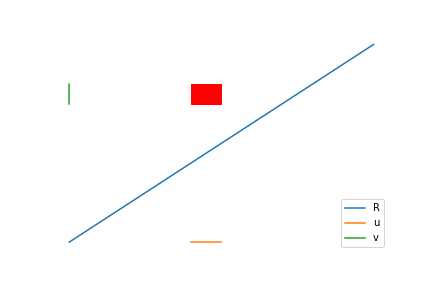
\includegraphics[width=0.90\textwidth]{graph_int.png}
\end{center}

\begin{Prop}
$G(p,n)$ is Hausdorff.
\end{Prop}

That is because $R$ is closed in $F(p,n) \times F(p,n)$, $(F(p,n) \times F(p,n)) \setminus R = R^{\complement}$ is open.
$\implies \forall (x,y) \in R^{\complement} $ there is a basic open set $u \times v$ containing $(x,y)$ s.t. $ (u \times v) \cap R = \emptyset 
\implies \forall x, y \text{ s.t. } (x,y) \not\in R, \exists$ u around x and v around y s.t. $u \cap v = \emptyset$
Thus for any two points $[x] \neq [y] \in \equivclass{F(p,n)}$ there exist disjoint neighborhood of $x$ and $y$ and $ \equivclass{F(2,4)}$ which is exactly the definition of Hausdorff property.
\newline
\begin{Prop}
   $G(p,n)$ is locally euclidean. 
\end{Prop}
Now that we have Hausdorff property and secound countable basis, we need to prove that every point lying on a manifold has a neighbourhood that is homeomorphic to an open in $\RR^n$.
Then we can claim that $G(p,n)$ is a manifold.
\newline
First we define charts. Take $A \in Mat_{n \times p} $ denote by $A_{k}$, ($ k \in \text{ all possible picks of p from the set } [1, \dots , n] $) the $p \times p$ minor, formed by the $k_1$th $\dots k_p$th rows of $A$.
The set
$$ U_{k} = \{ A \; | \; \det(A_{k}) \neq 0 \} \subset F(p,n)$$ is open, because its complement is closed. 
We also have that $\forall g \in GL(p)$ if $A \in U_{k}$ then $ Ag \in U_{k}$. 
Indeed, because $\det(Ag) = \det(A) \det(g)$, $\det( (Ag)_{i,j}) \neq 0$ which means $Ag$  will belong to a set $U_{k}$ 
Next, define
$$V_{k} = \equivclass{U_{k}} = \pi (U_{k}) \subset G(p,k)$$
The set $V_{k}$ is open since the equivalence relation is open. i.e. $\pi$ is an open map.
\newline
$U_k$ has a canonical representative $A \sim \widehat{A A_{k}^{-1}}$. $\widehat{\cdot}$ discards all the rows whose index is in $k$.
Similarly $V_k$ has a canonical representative: $[A] \sim [\widehat{A A_{k}^{-1}}] $

\begin{Ex}
Following the previous example consider $ [A] \in G(2,4)$.
If a minor $A_{2,4}$ is invertible we have that
$
[A] \sim [\widehat{A A_{2,4}^{-1}}] = 
\widehat{\begin{bmatrix}
* & * \\
1 & 0 \\
* & * \\
0 & 1
\end{bmatrix}} = \begin{bmatrix}  * & * \\ * & * \end{bmatrix}
$.
Since charts $ \bigcup U_k$ cover $F(p,n)$, charts $V_k$ cover $G(p,n)$ (because $\pi$ is open).
\end{Ex}
Now we define homeomorphisms between charts $V_k$ and opens in $R^{p \times (n-p)}$ as follows:
$$ \phi_{k}: V_{k} \subset G(p,n) \to Mat_{ (n-p) \times p} (\RR) \simeq \RR^{ (n-p) \times p) }, \quad \phi_{k}([A]) = \widehat{A A_{k}^{-1}} $$
We can show that $\phi$ is well defined. 
\newline
Let $A, A^\prime \in [A]$ we will show that $\phi$ is well defined. Equivalently $\phi_{k}(A) = \phi_{k}(A^\prime])$
Since $A$ and $A^\prime$ are in the same class, we have that $A^\prime = A g, \quad g \in GL(p) $, $\phi_{k}(A) = A A_{k}^{-1}$.
$$ \phi_{k}(A^\prime) = \phi_{k}(A g) = Ag ((Ag)_{k})^{-1} = Ag( A_{k} g )^{-1} = A g g^{-1} A_{k}^{-1} = A I A_{k}^{-1} = A A_{k}^{-1} = \phi_{k}(A) $$

$\phi$ is continuous because matrix multiplication is continous. Next, we can see that $\phi$ is surjective and $\phi^{-1}$ is continuous by explicitly defining inverse.

$$\phi_{k}^{-1}(\begin{pmatrix} \text{--- } \alpha_{1} \text{ ---}  \\ \vdots \\ \text{--- }  \alpha_{n-p} \text{ ---} \end{pmatrix}) =
\begin{pmatrix} 1_1 \\ \vdots  \\ 1_p \\ \alpha_1 \\ \vdots \\  \alpha_{n-p}  \end{pmatrix} $$
Finally, to show that $\phi$ is a homeomorphism,
we have left to shot that $\phi$ is injective. 
\newline
Assume that there $\phi_{k}$ is not injective then there are $A \in [A]$ and $B \in [B]$ such that there is \textbf{no} $g \in GL(p)$
for which $A g =  B$. i.e. $A A_{k}^{-1} = B B_{k}^{-1} \; \iff  \; 
 A A_{k}^{-1} B_{k} = B$ but $A_{k}^{-1} B_{k} \in GL(p)$ thus we reach contradiction.
Therefore $\phi_{k}$ is homeomorphism
\newline 
\begin{Ex} \label{ex1}
    Let $A = \begin{bmatrix}
        2 & 6 \\
        1 & 3 \\
        2 & 1 \\
        4 & 3 \\
    \end{bmatrix}, \quad [ A ] \in V_{3,4}$
    $$ A A_{3,4}^{-1} =  \begin{pmatrix} 2 & 6 \\ 1 & 3 \\ 2 & 1 \\ 4 & 3 \\ \end{pmatrix} \begin{pmatrix} \frac{3}{2} & -\frac{1}{2} \\ -2 & 1 \\ \end{pmatrix}
    = \begin{pmatrix} -9 & 5 \\ -\frac{9}{2} & \frac{5}{2} \\ 1 & 0 \\ 0 & 1 \end{pmatrix}
    $$
    the above multiplication is continuous by \ref{quotientTop} and we can exlcude rows $3$ and $4$ so that we get result in $R^4$.
    Then the restriction to $R^4$ is also continuous.
    $$ \phi_{3,4}([A]) = \begin{pmatrix} -9 & 5 \\ -\frac{9}{2} & \frac{5}{2} \end{pmatrix} $$
\end{Ex}
Next the inverse map  $\phi_{3,4}(\beta)^{-1} \; \beta \in Mat_{2 \times 2} = \phi_{3,4}(A_{1,2} A_{3,4}^{-1} g) = [A] $ for some matrix $A$, such that $A_{1,2} = \beta$.
But if we pick $g = A_{3,4}$ then 
$ \phi_{3,4}(\beta) =
\begin{bmatrix}
    \beta_{1,1} & \beta_{1,2} \\ 
    \beta_{2,1} & \beta_{2,2} \\
    1 & 0 \\ 
    0 & 1 \\
\end{bmatrix}
$
More generally
$$\phi_{i,j}^{-1} : \RR^4 \to v_{i,j} \subset G(2,4) \quad \phi_{i,j}^{-1}(\beta) \to 
\begin{bmatrix}
    \beta \\
    I_{2 \times 2}
\end{bmatrix} = [\alpha]
$$
Such that $\alpha [i:] = \beta[1:]$, $\alpha[j:] = \beta[2:]$ , $\alpha[ (I \setminus \{i,j\})[1] ] = I[1:]$ and
$\alpha[ (I \setminus \{i,j \})[2] ] = I[2:]$
\newline
\begin{Ex}
   $ \phi_{3,4}^{-1} (\alpha) = [A] $ as defined in \ref{ex1}
   $$ \phi_{3,4}^{-1}  \begin{pmatrix} -9 & 5 \\ -\frac{9}{2} & \frac{5}{2} \end{pmatrix} = \begin{bmatrix} -9 & 5 \\ -\frac{9}{2} & \frac{5}{2} \\ 1 & 0 \\ 0 & 1 \end{bmatrix} $$ 
   We can confirm that $ \alpha = \begin{bmatrix} -9 & 5 \\ -\frac{9}{2} & \frac{5}{2} \\ 1 & 0 \\ 0 & 1 \end{bmatrix}$ and $A = \begin{bmatrix}
        2 & 6 \\
        1 & 3 \\
        2 & 1 \\
        4 & 3 \\
    \end{bmatrix}$
    span the same subspace.
    Because if we take $g = \begin{pmatrix} 2 & 1 \\ 4 & 3 \\ \end{pmatrix}$
    then $\alpha g = A$
\end{Ex}
Since $\bigcup U_{i,j}$ covers $F(2,4)$, $\cup v_{i,j}$ covers $G(2,4)$
Finally, we check transition maps.
$$ \phi_{1,2}([A])^{-1} = A_{3,4} A_{1,2}^{-1}, \quad \phi_{1,2}^{-1}(u) =
\begin{pmatrix}
1 & 0 \\
0 & 1 \\
v_{1,1} & v_{1,2} \\
v_{2,1} & v_{2,2}
\end{pmatrix}
$$

$$ \phi_{2,4}([A]) = A_{1,3} A_{2,4}^{-1}, \quad \phi_{2,4}^{-1}(v) = 
\begin{pmatrix}
v_{1,1} & v_{1,2} \\
1 & 0 \\
v_{2,1} & v_{2,2} \\
0 & 1
\end{pmatrix}
$$
$$ \phi_{2,4} \circ \phi_{1,2}^{-1}(v) = 
\begin{pmatrix}
v_{1,1} & v_{1,2} \\
v_{2,1} & v_{2,2}
\end{pmatrix} =
\begin{pmatrix}
    1 & 0 \\
    v_{1,1} & v_{1,2}
\end{pmatrix}
\begin{pmatrix}
    0 & 1 \\
    v_{2,1} & v_{2,2}
\end{pmatrix} ^{-1}
= 
\begin{pmatrix}
    1 & 0 \\
    v_{1,1} & v_{1,2}
\end{pmatrix}
\begin{pmatrix}
    v_{2,2} & -1 \\
    -v_{2,1} & 0
\end{pmatrix} \frac{1}{-v_{2,1}} = 
$$
$$ -\frac{1}{v_{2,1}} \begin{pmatrix} v_{2,2} & -1 \\ v_{1,1} v_{2,2} - v_{1,2} v_{2,1} & -v_{4} \end{pmatrix}
$$
\newline
Now let's check the transition map $ \phi_{3,4} \circ \phi_{2,3}^{-1} $ 
$$ \phi_{3,4} \circ \phi_{2,3}^{-1} (v) =
\begin{pmatrix} v_{1,1} &  v_{1,2} \\ 1 & 0 \end{pmatrix} 
\begin{pmatrix} 0 & 1 \\ v_{2,1} & v_{2,2} \end{pmatrix} = 
-\frac{1}{v_{2,1}} \begin{pmatrix} v_{1,1} v_{2,2} + v_{1,2} v_{2,1} & -v_{1,1} \\ v_{2,2} & -1 \end{pmatrix}
$$ 
Hence $G(p,n)$ can be equipped with the structure of a $p (n-p) $ dimensional smooth manifold.
\section{Grassmann manifold as a quotient manifold }
\section{Grassman manifold as a set of projectors }

\chapter{Optimization Algorithms}
\section{Gradient Descent}
\section{Newton 1}
\section{Newton 2}

\chapter{Solve Rayleigh Quotient}
\section{Gradient Descent}
\section{Newton 1}
\section{Newton 2}
 
\chapter{ONE MORE?} 

\chapter{Notation} 
 
\noindent\begin{tabularx}{\textwidth}{@{}XXX@{}}  \toprule
  Symbol & Matrix Definition & Name \\
  \toprule
  $F(p,n)$  & $\{A \in Mat_{n \times p}  \; | \; rkA = p  \} $ & 2 frames \\
  \toprule
  $St(p,n)$ & $ \{ A \in F(2,4) \; | \; A^T A = I_k \} $ & Stiefel Manifold \\
  \toprule
  $ GL(p)$ &  $ \{ A \in Mat_{n \times n} \; | \; det A \neq 0 \}$ & General Linear Group \\
\end{tabularx}\offinterlineskip

 
\bibliographystyle{alpha}
\bibliography{biblio}
 
 

\end{document}          
